\section{End-to-End Benchmarks}
\label{s:benchmarks}

We start by evaluating the total cost attributable to all mitigations for transient execution attacks.
This value is different for each individual CPU, so we compare both across generations of processors and between vendors.

Later sections will go into more detail on how individual attacks work and the characteristics of their respective mitigations, but for now we wish only to gain a high level understanding of which mitigations are relevant from a performance perspective.

The primary impact of transient execution attacks is to leak information across protection boundaries.
Accordingly mitigations to prevent such leakage often involve extra operations when the CPU transitions from one protection domain to another.
Alternatively, some mitigations must be enabled continuously while untrusted code is being executed.
Based on this, we focus on two particularly relevant protection boundaries: the user-kernel interface for the operating system, and the sandboxing that web browsers' JavaScript engines provide between execution contexts for different sites.
The boundary between a hypervisor and its guest operating system is also notable, but we did not find significant performance differences between running virtualization workloads with and without mitigations enabled.

In addition, we consider the case of a compute-intensive workload running within a single operating system process.
That involves no protection boundary crossings, and thus measures only the impact of mitigations the operating system keeps enabled all the time.

\subsection{Methodology}
In the following benchmarks we evaluate across seven different CPU microarchitectures from two vendors.
Considering different microarchictures enables us to observe design improvements between successive releases.
Table~\ref{fig:cpus} lists out detailed information on each CPU.

\begin{table*}[t]
    \begin{center}
    \begin{tabular}{ cllcccc }
      \textbf{Vendor} & \textbf{Model} & \textbf{Microarchitecture} & \textbf{Power (W)} & \textbf{Clock (GHz)} & \textbf{Cores} \\ \hline 
        \multirow{5}{*}{Intel} & E5-2640v4         & Broadwell (2014)          & 90 & 2.4 & 10 \\
                               & i7-6600U          & Skylake Client (2015)   & 15 & 2.6 & 2 \\
                               & Xeon Silver 4210R & Cascade Lake (2019)       & 100 & 2.4 & 10 \\
                               & i5-10351G1        & Ice Lake Client (2019)  & 15 & 1.0 & 4 \\
                               & Xeon Gold 6354    & Ice Lake Server (2021)  & 205 & 3.0 & 18 \\ \hline
        \multirow{3}{*}{AMD}   & Ryzen 3 1200      & Zen (2017)                & 65 & 3.1 & 4 \\
                               & EPYC 7452         & Zen 2 (2019)              & 155 & 2.35 & 32 \\
                               & Ryzen 5 5600X     & Zen 3 (2020)              & 65 & 3.7 & 6 \\ \hline
    \end{tabular}
    \end{center}
    \caption{Information about each of the CPUs we evaluate. All except the Ryzen 3 1200 have 2-way SMT ("hypertheads" in Intel terminology).}
    \label{fig:cpus}
  \end{table*}

The processors we evaluate span from before the discovery of Spectre and Meltdown (Broadwell, Skylake Client, and Zen) to the most recently available Intel mobile and server microarchictures (Ice Lake Client and Server respectively) and AMD microarchicture (Zen~3).
Despite sharing the same name, Ice Lake Client and Ice Lake Server differ meaningfully from one another.
All machines have an up-to-date kernel: either version 5.11, the 5.14 release, or the 5.4 long-term maintenance release.

This diversity of systems gives a broad view of the ecosystem, but at the same time our work is complicated by all the different dimensions they vary on.
Our processors range from 1.0 GHz to 3.7 Ghz and from 2 cores to 32 cores.
Newer ones incorporate not just design improvements, but also tend to have smaller transistors, faster RAM, and so forth.
For these reasons our experiments focus primarily on relative differences between configurations of the same machine.

To measure the impact of individual mitigations, we run  Linux with the default set of mitigations enabled, and then use kernel boot parameters to successively disable them to determine the overhead that each one causes.
Some mitigations are applied separately by Firefox, which we control via its \texttt{about:config} interface.
Since variability within runs frequently exceed the total overheads we are measuring, we average the times from several hundred runs of each configuration.


\subsection{LEBench}

\begin{figure}[t]
    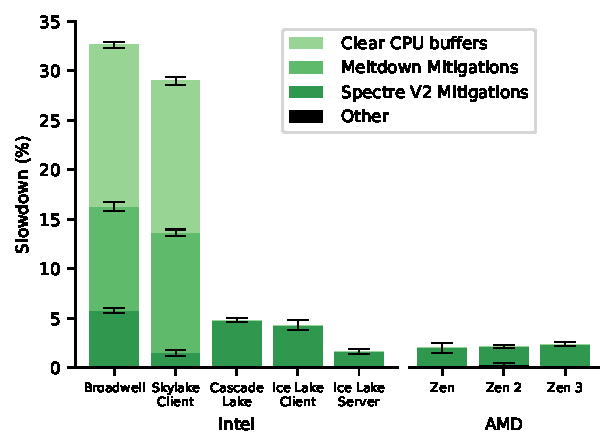
\includegraphics[width=\columnwidth]{plots/lebench.pdf}
    \caption{The overhead of mitigations on the LEBench benchmark suite which stresses the operating system interface.}
    \label{fig:lebench}
\end{figure}


LEBench~\cite{ren:lebench} is a collection of microbenchmarks for measuring specific operating system operations.\footnote{To align with experiments from elsewhere in this thesis, we use the version of the LEBench benchmarks distributed with \sys~\cite{behrens:ward} .}
In this experiment, we track the geometric mean of benchmarks from the suite.
As seen in Figure~\ref{fig:lebench} the overhead has decreased sharply for newer processors:
CPUs which incorporate hardware mitigations (for Intel) or from a vendor whose CPUs were not vulnerable to all attacks in the first place (AMD) exhibit substantially smaller overheads.

Also notable is that only a small number of mitigations are responsible for nearly all of the overheads.
Collectively, all unlisted mitigations caused a fraction of a percent slowdown on Zen 2, but on our other processors had no statistically significant impact at all.

\subsection{Octane 2}

\begin{figure}[t]
    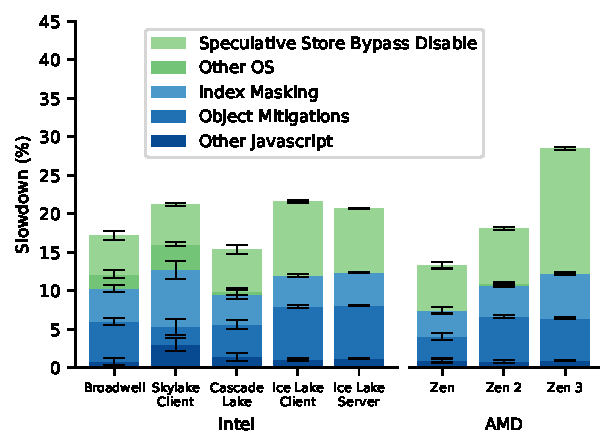
\includegraphics[width=\columnwidth]{plots/octane2.pdf}
    \caption{Slowdown on the Octane 2 browser benchmark caused by JavaScript and operating system level mitigations.}
    \label{fig:octane2}
\end{figure}

Octane 2 is a benchmark for JavaScript performance, which we run from within Firefox.
Figure~\ref{fig:octane2} plots the percent decrease in scores caused by enabling each mitigation in turn.
JavaScript mitigations (Index masking, object mitigations, and ``other JavaScript'') are shown in blue, while operating system controlled mitigations including Speculative Store Bypass Disable (SSBD) and ``other OS'' are shown below them in green.

All JavaScript mitigations are implemented by the JIT engine inserting extra instructions into the generated instruction stream, and are used to prevent different variations of the Spectre V1 attack.
For instance, index masking ensures that speculative accesses to an array do not index past the end of an array.
It does so by placing a conditional move instruction before every array access which checks whether the access is in bounds and overwrites the index with zero otherwise.
This check overall takes very little time but it prevents the CPU from starting to pull the array contents into cache until the array length is known.
Across many millions of array accesses in the Octane 2 benchmark, this ends up causing a non-trivial cost.

Speculative Store Bypass Disable is an OS level mitigation that is disabled by default for most processes, but which Firefox specifically opts into.
It does so to provide stronger sandboxing of JavaScript execution.
Intel has reserved a bit in in the \texttt{ARCH\_CAPABILITIES} model-specific register to indicate that a given processor isn't vulnerable to Speculative Store Bypass and therefore that the associated mitigation is neither needed nor implemented.
However, we do not know of any CPUs for either vendor that set that bit, not even models that came out years after the attack was discovered.

\subsection{Virtual Machine Workload}

We also measure the performance of running LEBench inside of a KVM virtual machine with and without host mitigations enabled.
This lets us see whether mitigations on the host impact performance observed by the guest.
In our experiments the measured overhead was $\pm 3$\% on all systems, signalling that the mitigations applied by a virtual machine monitor do no significantly impact the performance here.
Some runs suggested a slowdown in the range of 1-3\%, but our methodology resulted in too much variability between runs to be confident whether or not that was caused by noise. 
In any case, we were unable to attribute the slowdown to specific mitigations.

\subsection{Swaptions}
\label{sec:parsec}
As a final benchmark we measure the overhead of running swaptions, one of the benchmarks from the PARSEC suite.
It involves neither significant numbers of calls into the operating system nor user-level sandboxing, as explored by the previous benchmarks, which makes it ideal to measure the impact solely of ``always on'' mitigations that the OS applies to running processes.

We are unable to observe any meaningful difference between running with and without the default set of mitigations.
On all our tested systems, the results for the two configurations are within a fraction of a percent.
This matches prior reports that compute intensive workloads without interactions with the OS do not suffer much from mitigations, and serves as a reminder that slowdowns from transient execution attack mitigations aren't relevant to all workloads.

The one exception is that when we force-enable mitigations for Speculative Store Bypass, we observe significant overheads.
\S\ref{sec:ssb} explores those overheads in more detail.

\subsection{Summary}
Each of these benchmarks plots a very different trajectory of mitigation costs.
Workloads that stress the operating system interface have received the most attention, and overheads on LEBench have gone from over 30\% on older Intel CPUs to under 3\% on the latest models from both vendors.
By contrast, JavaScript overhead has been consistently in the range of 15\% to 25\%, with the newest AMD processor we tested paying an even larger cost.
Our compute-intensive benchmark has negligible overhead regardless of the processor.
